% ============================================================
% Chương 5. Thiết kế cơ sở dữ liệu  (chuẩn 1.1, 1.2, 2.2)
% Nguồn: docs/design_levels.md, docs/contract.md, docs/data_models.md
% ============================================================
\section{Thiết kế cơ sở dữ liệu}
\label{sec:thiet-ke}

Cơ sở dữ liệu của hệ thống được thiết kế qua ba mức. Mức ý niệm xác định các thực thể nghiệp
vụ và quan hệ giữa chúng, độc lập với cách lưu trữ. Mức luận lý tổ chức các thực thể đó
thành bảng, cột, khóa và xác định độ chi tiết (grain) của từng bảng. Mức vật lý quyết định
cách các bảng được lưu và truy cập trên từng hệ quản trị cụ thể. Giữa mức ý niệm và mức luận
lý, dữ liệu nguồn được phân tích theo phụ thuộc hàm để đưa về dạng chuẩn, sau đó được phi
chuẩn hóa có chủ đích thành dimensional model. Cuối chương trình bày các mô hình dữ liệu phi
quan hệ được hiện thực trên cùng bộ dữ liệu và kết quả so sánh với mô hình quan hệ.

% ------------------------------------------------------------
\subsection{Mức ý niệm}
\label{sec:y-niem}

Ở mức ý niệm, dữ liệu OULAD được mô tả bằng tám thực thể (Hình~\ref{fig:erd},
Bảng~\ref{tab:thuc-the}). Năm thực thể đầu là các đối tượng nghiệp vụ; ba thực thể sau là
quan hệ nhiều-nhiều giữa chúng, mỗi quan hệ mang thuộc tính riêng nên được mô hình hóa thành
thực thể kết hợp.

Sơ đồ có bốn thực thể yếu. Đợt học là thực thể yếu của Học phần, khóa riêng phần là mã kỳ
(kỳ 2013J có nhiều học phần cùng mở). Đăng ký và Lần nộp được xác định bằng khóa của hai thực
thể chủ; Lượt truy cập có thêm khóa riêng phần là ngày, vì một sinh viên mở cùng một học liệu
vào nhiều ngày.

\begin{figure}[htbp]
\centering
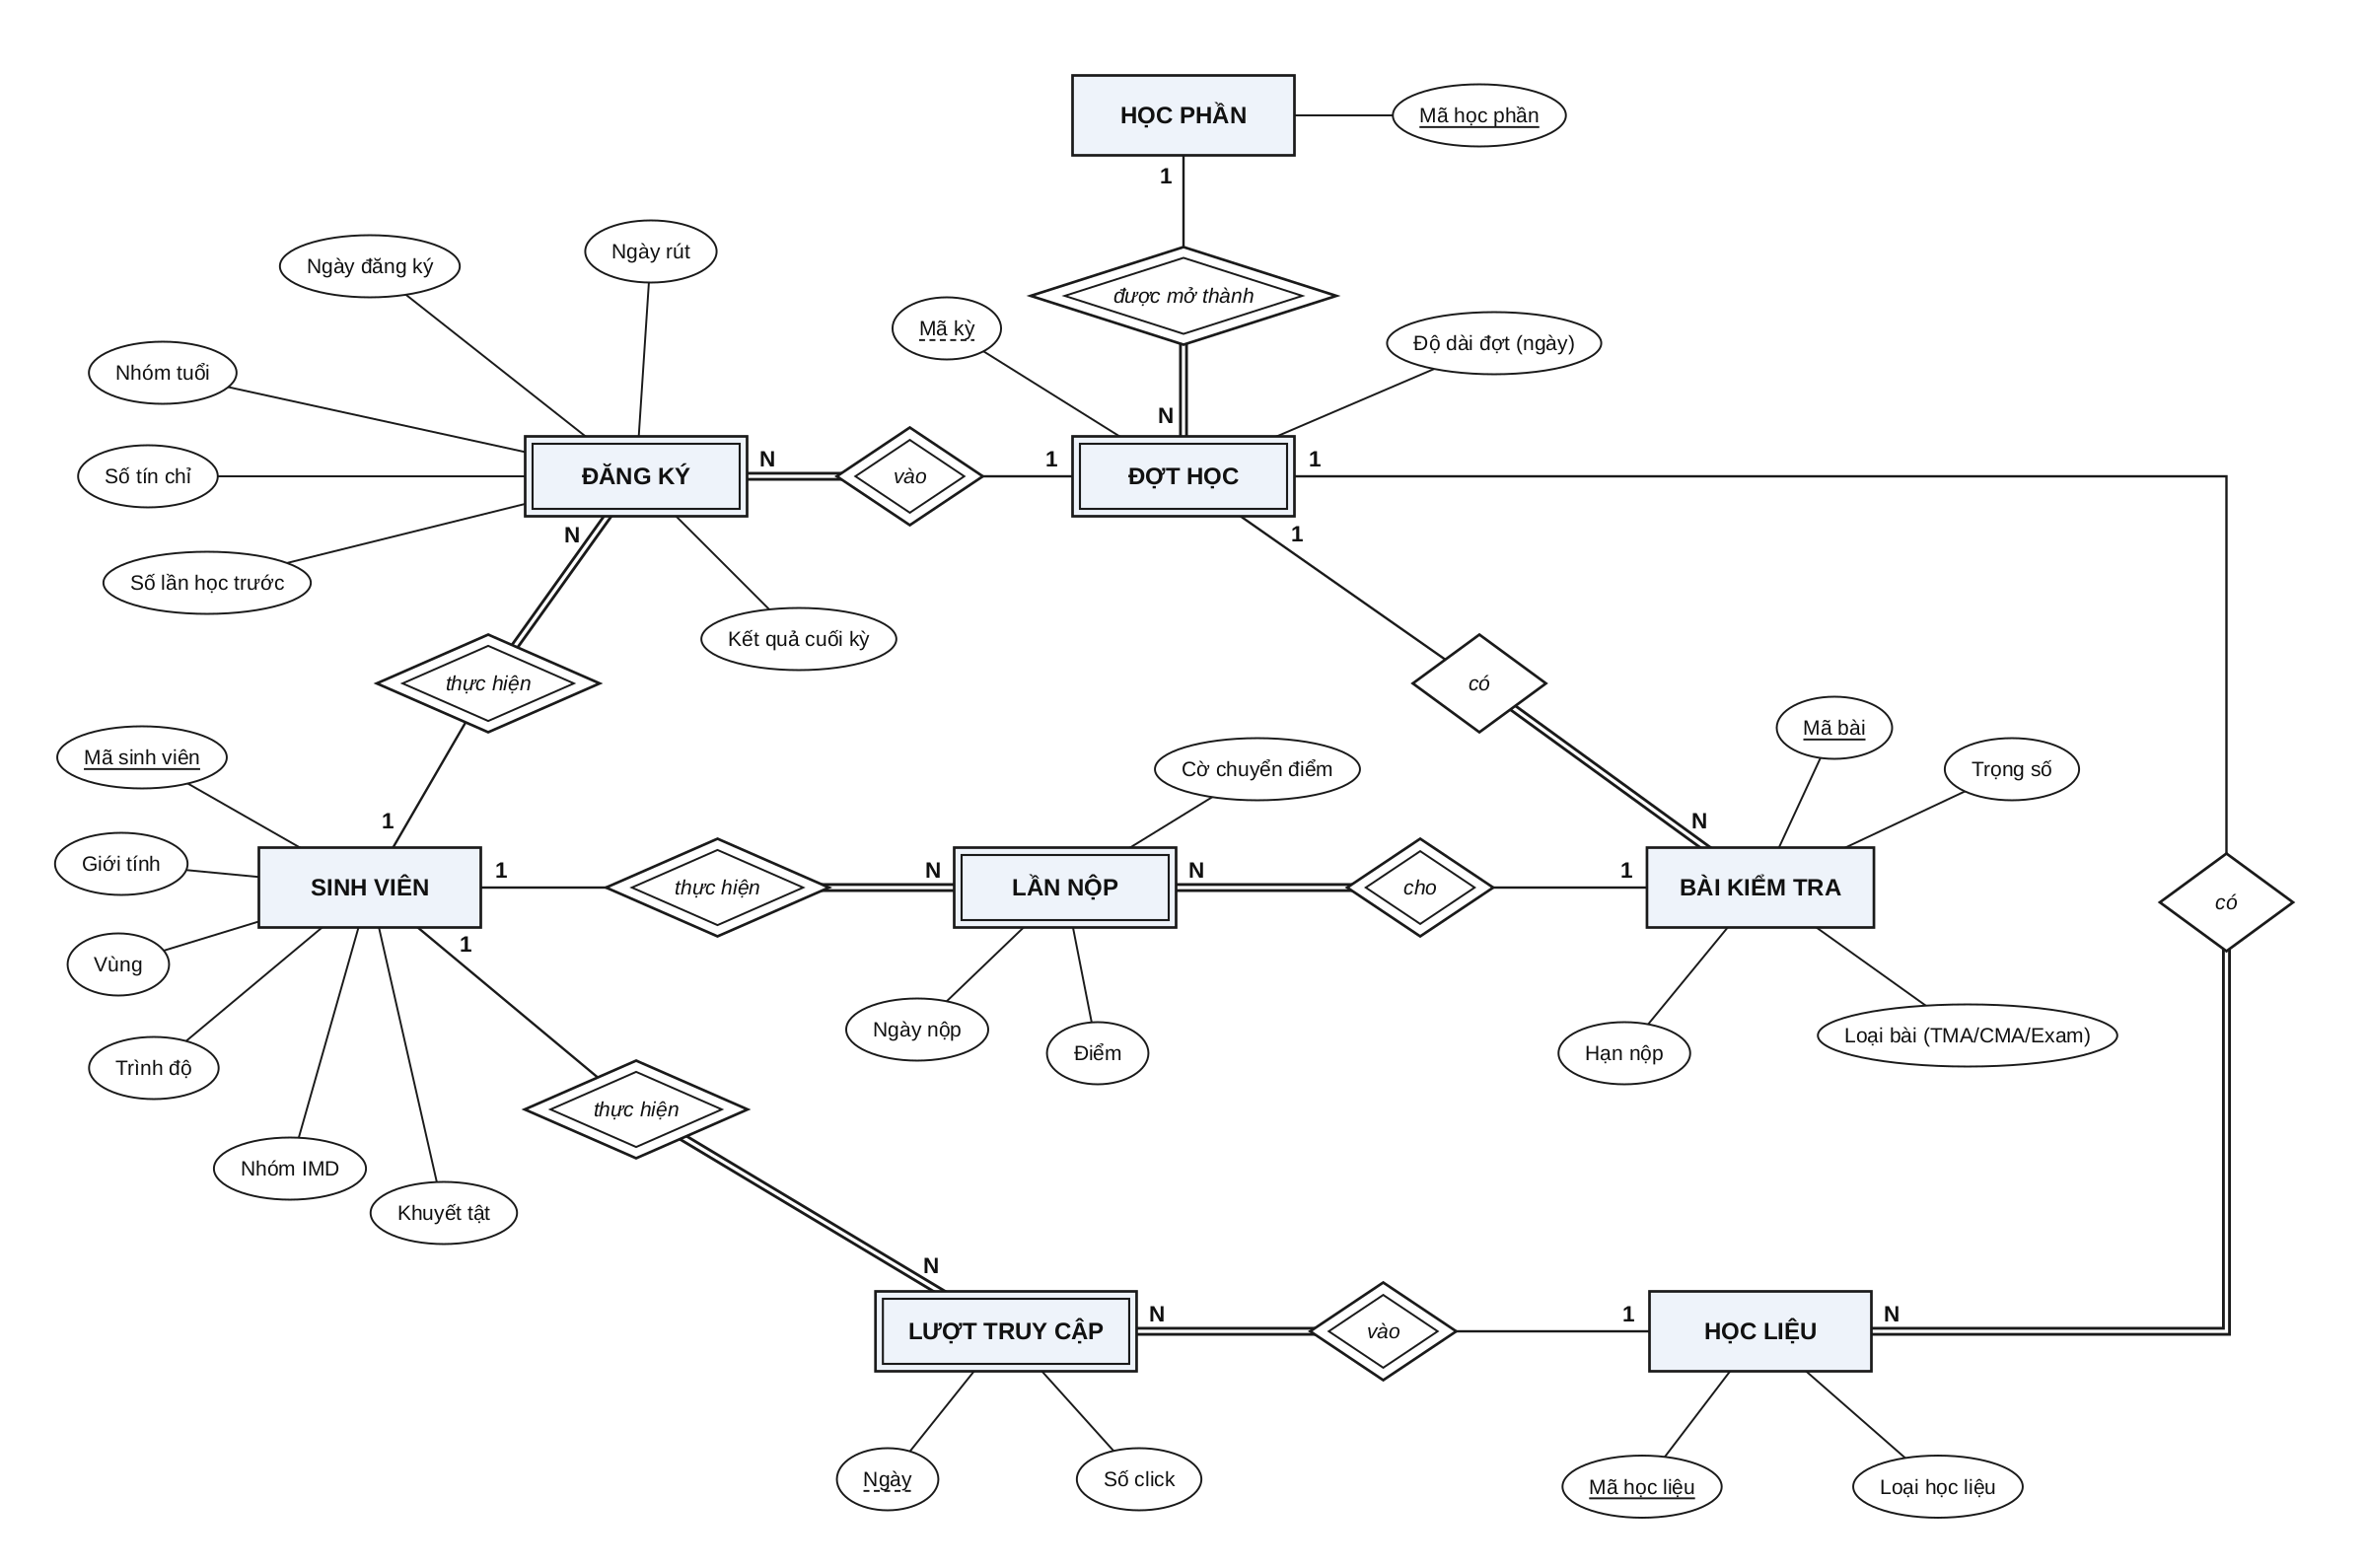
\includegraphics[width=0.9\textwidth]{Images/erd_y_niem.png}
\caption{Sơ đồ thực thể -- mối quan hệ ở mức ý niệm}
\label{fig:erd}
\end{figure}

\begin{table}[htbp]
\centering
\small
\begin{tabularx}{\textwidth}{|p{2.4cm}|X|X|}
\hline
\textbf{Thực thể} & \textbf{Ý nghĩa nghiệp vụ} & \textbf{Thuộc tính chính} \\ \hline
Học phần & Một môn học (7 môn, ký hiệu AAA đến GGG) & Mã học phần \\ \hline
Đợt học & Một lần mở học phần trong một kỳ (22 đợt) & Mã kỳ, độ dài đợt (ngày) \\ \hline
Sinh viên & Người học & Giới tính, vùng, trình độ, nhóm IMD, tình trạng khuyết tật \\ \hline
Bài kiểm tra & Bài TMA, CMA hoặc Exam của một đợt & Loại bài, hạn nộp, trọng số \\ \hline
Học liệu & Một tài nguyên trên VLE của một đợt & Loại học liệu \\ \hline
Đăng ký & Quan hệ Sinh viên -- Đợt học & Ngày đăng ký, ngày rút, nhóm tuổi, số tín chỉ, số lần học trước, kết quả cuối kỳ \\ \hline
Lần nộp & Quan hệ Sinh viên -- Bài kiểm tra & Ngày nộp, điểm, cờ chuyển điểm \\ \hline
Lượt truy cập & Quan hệ Sinh viên -- Học liệu theo ngày & Ngày, số click \\ \hline
\end{tabularx}
\caption{Thực thể ở mức ý niệm}
\label{tab:thuc-the}
\end{table}

Sơ đồ thể hiện các quy tắc nghiệp vụ sau, và mức luận lý, mức vật lý phải giữ đúng các quy tắc này:
\begin{itemize}
  \item Một sinh viên có thể đăng ký nhiều đợt, kể cả học lại cùng một học phần.
  \item Một lượt đăng ký có thể bị rút, kể cả trước ngày khai giảng.
  \item Mỗi bài kiểm tra và mỗi học liệu thuộc đúng một đợt; mã học liệu không dùng lại giữa
        các đợt.
  \item Mỗi sinh viên nộp mỗi bài nhiều nhất một lần; điểm có thể được chuyển từ đợt trước.
\end{itemize}

Quyết định quan trọng nhất ở mức này là đặt mỗi thuộc tính vào đúng thực thể. File
\texttt{studentInfo} gộp thuộc tính của Sinh viên và của Đăng ký trên cùng một dòng
(mục~\ref{sec:van-de-du-lieu}). Kiểm tra trên dữ liệu cho thấy giới tính, vùng, trình độ, nhóm
IMD và tình trạng khuyết tật không đổi giữa các đợt của cùng một sinh viên, nên thuộc về Sinh
viên. Nhóm tuổi thì khác: nó thay đổi giữa các lần đăng ký ở 72 sinh viên, nên thuộc về Đăng
ký. Nếu gán nhóm tuổi cho Sinh viên, 72 sinh viên này sẽ bị ghi sai nhóm tuổi ở một số đợt.

% ------------------------------------------------------------
\subsection{Chuẩn hóa dữ liệu nguồn}
\label{sec:chuan-hoa}

Mục này trình bày chuẩn hóa lược đồ: tách bảng theo phụ thuộc hàm để mỗi dữ kiện chỉ được
lưu ở một nơi. Đây là nghĩa khác với chuẩn hóa giá trị (đổi ký hiệu thiếu thành \texttt{NULL},
thống nhất cách ghi, đặt kiểu dữ liệu), vốn là một bước làm sạch trong ETL (mục~\ref{sec:etl}).

Bảng~\ref{tab:phu-thuoc-ham} liệt kê các phụ thuộc hàm của dữ liệu nguồn và dạng chuẩn bị vi
phạm. Các phụ thuộc hàm này được kiểm chứng trên dữ liệu staging chứ không chỉ suy ra từ tên
cột; mỗi phụ thuộc hàm có một bài kiểm thử, nên nếu dữ liệu nguồn thay đổi làm một phụ thuộc
hàm không còn đúng, bộ kiểm thử sẽ báo lỗi.

\begin{table}[htbp]
\centering
\footnotesize
\begin{tabularx}{\textwidth}{|p{2.7cm}|X|p{2.7cm}|p{1.2cm}|p{2.7cm}|}
\hline
\textbf{Bảng nguồn} & \textbf{Phụ thuộc hàm} & \textbf{Kiểm chứng trên dữ liệu} & \textbf{Vi phạm} & \textbf{Xử lý} \\ \hline
\texttt{studentVle} & Không có khóa: (sinh viên, đợt, học liệu, ngày) lặp lại & 3.810.465 dòng trùng khóa & 1NF & Gộp thành một dòng mỗi khóa, cộng số click \\ \hline
\texttt{studentInfo} & \texttt{id\_student} $\rightarrow$ giới tính, vùng, trình độ, nhóm IMD, khuyết tật & Không sinh viên nào có hơn một giá trị (3.538 sinh viên học nhiều đợt) & 2NF & Tách thành bảng sinh viên \\ \hline
\texttt{studentInfo} & (sinh viên, đợt) $\rightarrow$ nhóm tuổi, số lần học trước, số tín chỉ, kết quả cuối kỳ & Nhóm tuổi đổi ở 72 sinh viên & Không & Giữ ở bảng đăng ký \\ \hline
\texttt{studentVle} & \texttt{id\_site} $\rightarrow$ mã đợt & Không học liệu nào thuộc hơn một đợt & 2NF & Bỏ mã đợt khỏi bảng click \\ \hline
\texttt{studentAssessment} & \texttt{id\_assessment} $\rightarrow$ mã đợt (qua \texttt{assessments}) & Không bài nào thuộc hơn một đợt & Không & Đã đạt 3NF \\ \hline
Cột suy ra & Ngày $\rightarrow$ tuần; đợt $\rightarrow$ độ dài đợt $\rightarrow$ hạn nộp bị thiếu & Theo công thức & 3NF & Bỏ cột, tính lại khi truy vấn \\ \hline
\end{tabularx}
\caption{Phụ thuộc hàm của dữ liệu nguồn và dạng chuẩn bị vi phạm}
\label{tab:phu-thuoc-ham}
\end{table}

Tách bảng theo đúng các phụ thuộc hàm trên cho ra một lược đồ đạt 3NF, trong đó bảng click
và bảng nộp bài không còn chứa mã đợt và số tuần; các thông tin này được tra qua bảng
dimension khi cần. Lược đồ 3NF này được hiện thực và dùng làm một trong các phương án so sánh
hiệu năng (chương~\ref{sec:danh-gia}).

Kho dữ liệu chính không dùng nguyên lược đồ 3NF mà phi chuẩn hóa có chủ đích ở ba điểm.
Thứ nhất, mã đợt được giữ trong bảng click và bảng nộp bài, để lọc theo một đợt mà không cần
phép nối và để gom cụm bảng click theo đợt. Thứ hai, số tuần được lưu sẵn trong mọi bảng
fact, để tổng hợp theo tuần và phân vùng bảng tiến độ theo tuần. Thứ ba, một số cột tổng hợp
được tính sẵn, như tổng click và số bài đã nộp của mỗi lượt đăng ký, cùng toàn bộ bảng tiến
độ theo tuần. Cái giá của các lựa chọn này là dữ liệu dư thừa: trên PostgreSQL, bảng click của kho chiếm
816 MB, lớn hơn bản 3NF (618 MB) khoảng 32\%. Dư thừa thường dẫn đến bất thường khi cập nhật
(update anomaly), nhưng vấn đề này không phát sinh ở đây: kho không bị sửa từng dòng mà được
dựng lại toàn bộ từ dữ liệu nguồn ở mỗi lần nạp, nên các cột dư thừa luôn được tính lại cùng
lúc. Để phát hiện trường hợp chính pipeline tính sai các cột này, bộ kiểm thử của nhóm còn
kiểm tra số tuần và các cột tổng hợp khớp với dữ liệu nguồn sau mỗi lần dựng kho.

% ------------------------------------------------------------
\subsection{Mức luận lý}
\label{sec:luan-ly}

Từ mô hình ý niệm, nhóm dựng kho theo dimensional model~\cite{kimball2013}:
\begin{enumerate}
  \item Lấy ba quan hệ nhiều-nhiều Đăng ký, Lần nộp, Lượt truy cập làm ba bảng fact, và thêm
        bảng tiến độ theo tuần cho cảnh báo sớm (BR4) và theo dõi tiến độ (BR7).
  \item Chốt grain của từng bảng fact trước khi chọn cột (Bảng~\ref{tab:grain}): bảng click gộp
        về mức sinh viên $\times$ học liệu $\times$ ngày, bảng tiến độ là lượt đăng ký $\times$ tuần.
  \item Lấy Đợt học, Sinh viên, Bài kiểm tra, Học liệu làm dimension; gộp Học phần vào dimension
        đợt học vì chỉ có mã; thêm dimension tuần vì mọi yêu cầu nghiệp vụ đều phân tích theo tuần.
  \item Chọn số đo cho từng bảng fact (Bảng~\ref{tab:so-do-fact}).
\end{enumerate}

Kết quả là một fact constellation, tức nhiều star schema dùng chung dimension: bốn bảng fact
dùng chung năm conformed dimension (Hình~\ref{fig:star}, Bảng~\ref{tab:grain}), nên số liệu giữa
các yêu cầu nghiệp vụ khớp nhau. Các phần sau gọi tắt lược đồ này là star.

\begin{figure}[htbp]
\centering
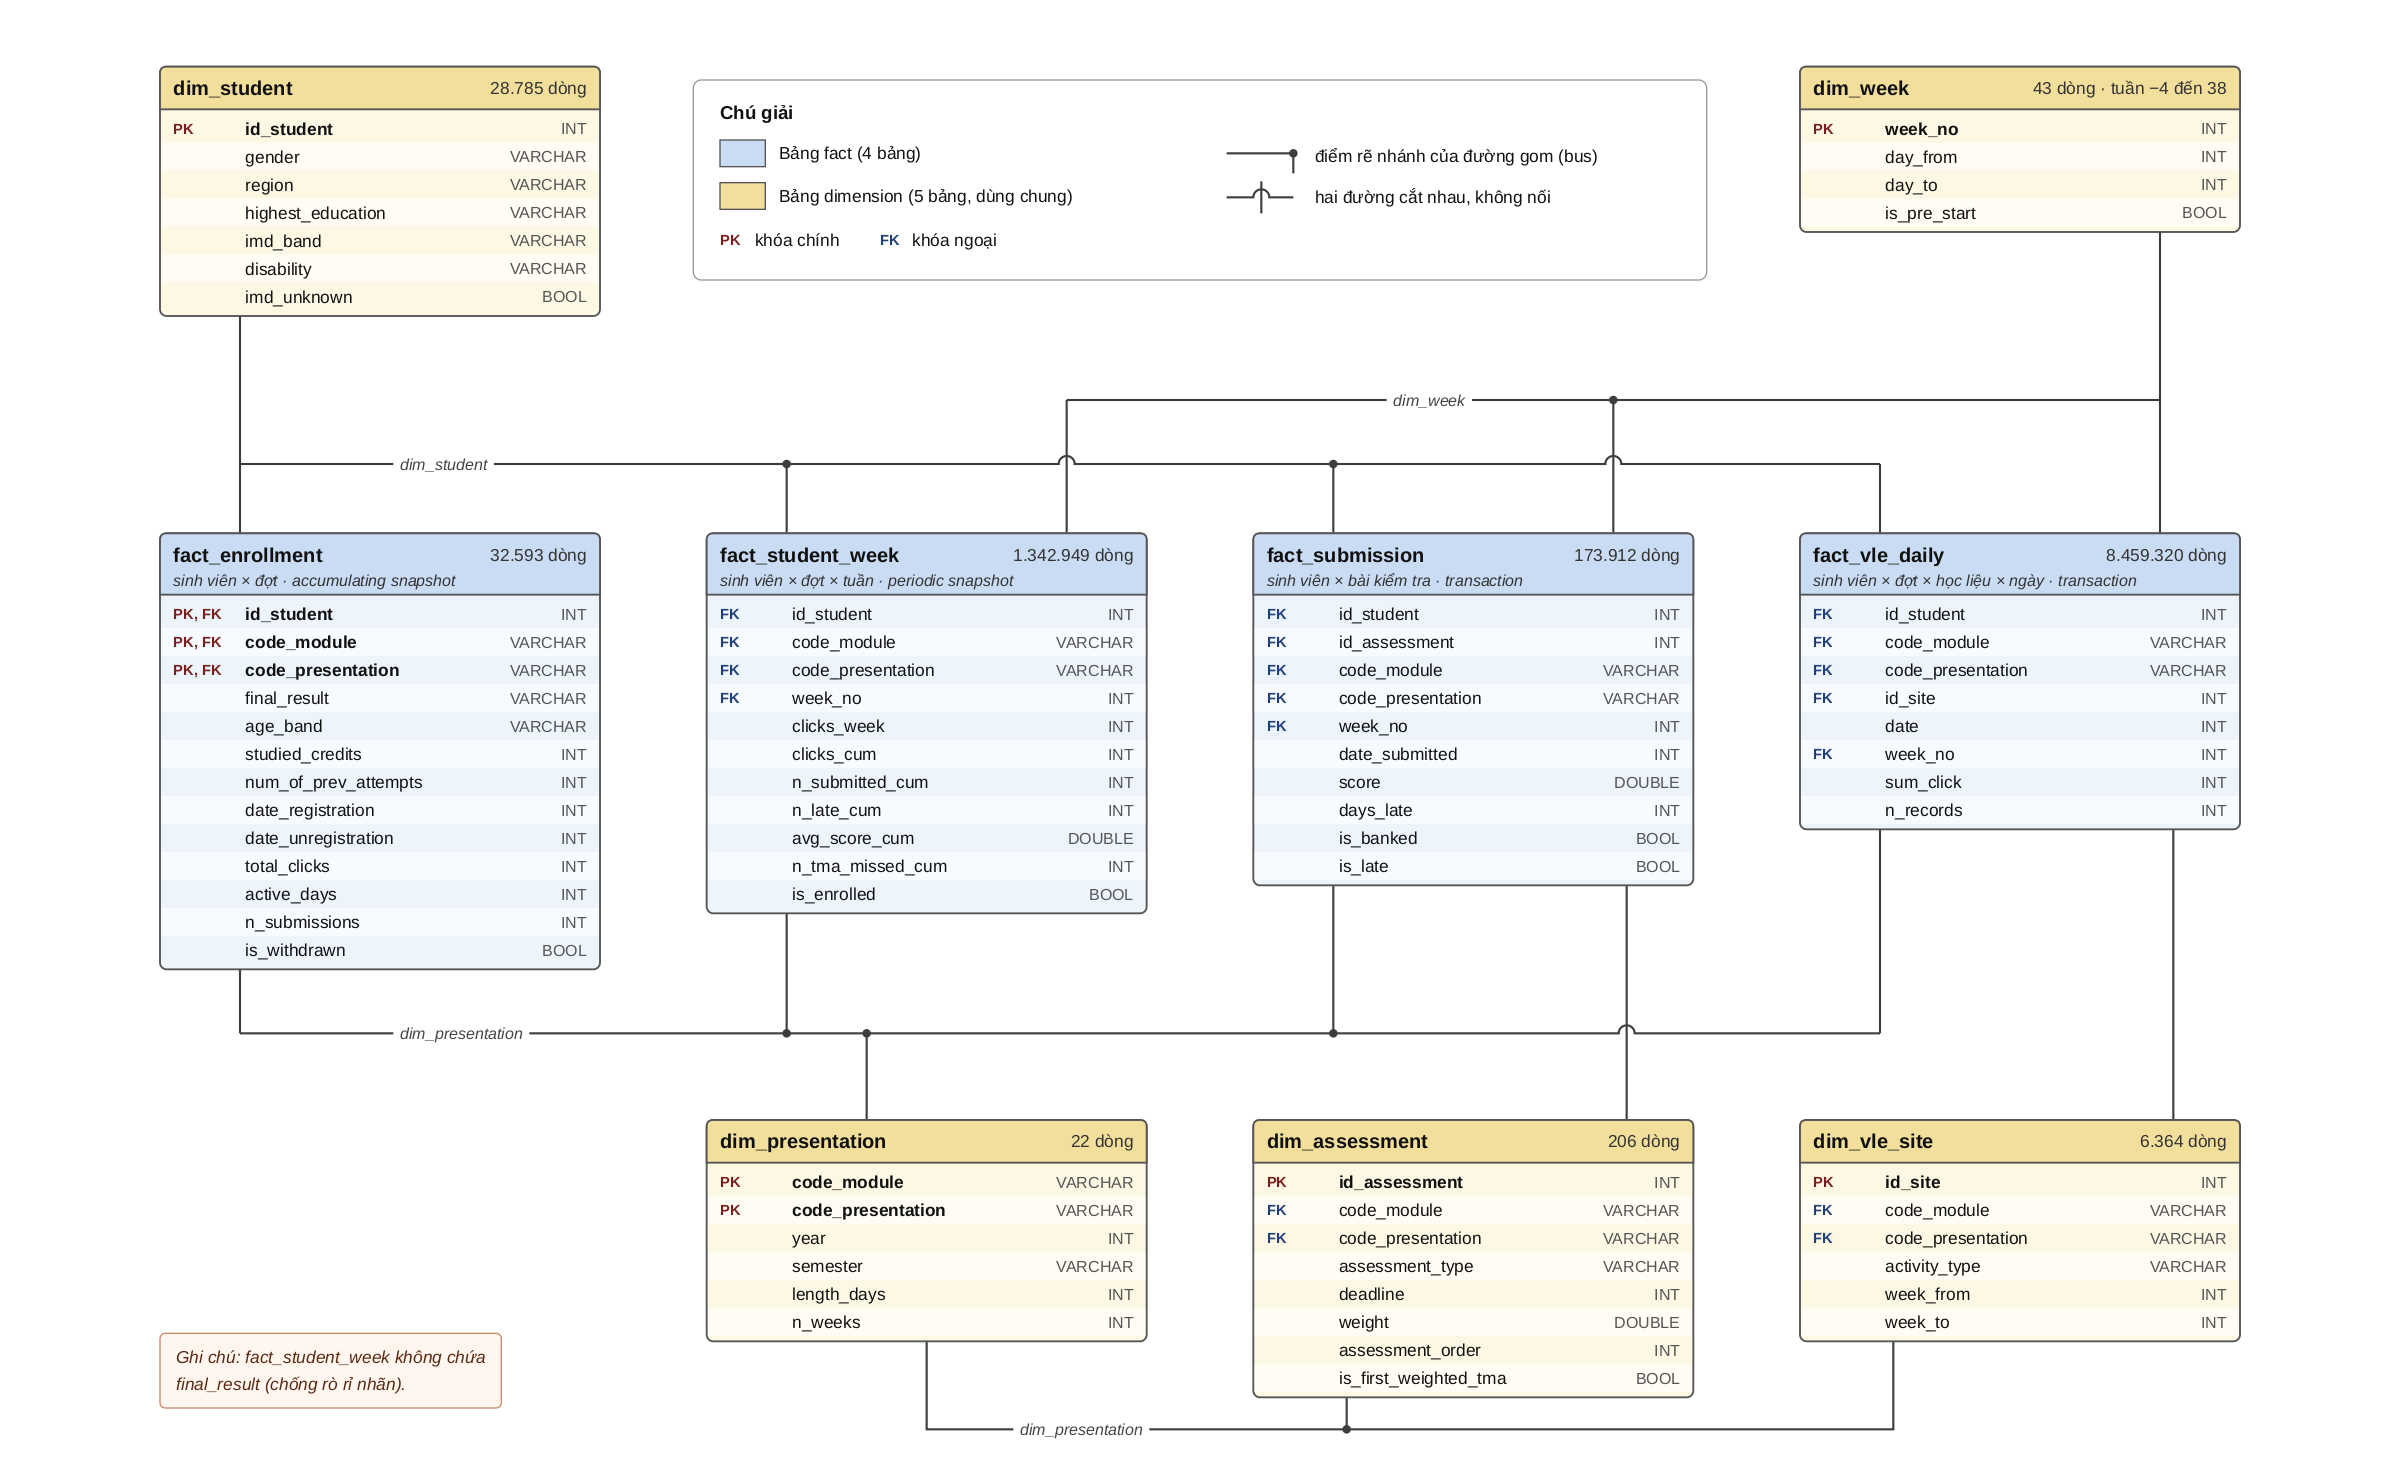
\includegraphics[width=\textwidth]{Images/star_schema.png}
\caption{Lược đồ kho dữ liệu: bốn bảng fact dùng chung năm bảng dimension}
\label{fig:star}
\end{figure}

Chi tiết của lược đồ được tóm tắt trong ba bảng: grain và số dòng của chín bảng
(Bảng~\ref{tab:grain}), thuộc tính chính của các dimension (Bảng~\ref{tab:thuoc-tinh-dim}), và
khóa dimension cùng số đo của các fact (Bảng~\ref{tab:so-do-fact}).

\begin{table}[htbp]
\centering
\small
\begin{tabularx}{\textwidth}{|l|X|l|r|}
\hline
\textbf{Bảng} & \textbf{Grain (một dòng là)} & \textbf{Loại} & \textbf{Số dòng} \\ \hline
\texttt{dim\_presentation} & một đợt học & dimension & 22 \\ \hline
\texttt{dim\_student} & một sinh viên & dimension & 28.785 \\ \hline
\texttt{dim\_assessment} & một bài kiểm tra & dimension & 206 \\ \hline
\texttt{dim\_vle\_site} & một học liệu & dimension & 6.364 \\ \hline
\texttt{dim\_week} & một tuần học, từ tuần $-4$ đến 38 & dimension & 43 \\ \hline
\texttt{fact\_enrollment} & sinh viên $\times$ đợt & accumulating snapshot & 32.593 \\ \hline
\texttt{fact\_vle\_daily} & sinh viên $\times$ đợt $\times$ học liệu $\times$ ngày & transaction & 8.459.320 \\ \hline
\texttt{fact\_submission} & sinh viên $\times$ bài kiểm tra & transaction & 173.912 \\ \hline
\texttt{fact\_student\_week} & sinh viên $\times$ đợt $\times$ tuần & periodic snapshot & 1.342.949 \\ \hline
\end{tabularx}
\caption{Các bảng của kho, grain và số dòng}
\label{tab:grain}
\end{table}

Bảng click (\texttt{fact\_vle\_daily}) là transaction fact nhưng được gộp ở mức ngày. Bảng tiến
độ theo tuần (\texttt{fact\_student\_week}) là periodic snapshot có đủ mọi tuần của lượt đăng ký, kể cả tuần không có hoạt động, để các dấu hiệu như
``không click trong 2 tuần gần nhất'' tính được trực tiếp.

\begin{table}[htbp]
\centering
\small
\begin{tabularx}{\textwidth}{|l|l|X|}
\hline
\textbf{Dimension} & \textbf{Khóa} & \textbf{Thuộc tính chính} \\ \hline
\texttt{dim\_presentation} & mã môn, mã kỳ & năm, kỳ (B hoặc J), độ dài đợt, số tuần \\ \hline
\texttt{dim\_student} & \texttt{id\_student} & giới tính, vùng, trình độ, nhóm IMD, khuyết tật \\ \hline
\texttt{dim\_assessment} & \texttt{id\_assessment} & đợt học, loại bài, hạn nộp, trọng số, thứ tự trong đợt \\ \hline
\texttt{dim\_vle\_site} & \texttt{id\_site} & đợt học, loại học liệu (20 loại) \\ \hline
\texttt{dim\_week} & \texttt{week\_no} & ngày bắt đầu, ngày kết thúc của tuần \\ \hline
\end{tabularx}
\caption{Thuộc tính chính của các bảng dimension}
\label{tab:thuoc-tinh-dim}
\end{table}

\begin{table}[htbp]
\centering
\small
\begin{tabularx}{\textwidth}{|l|p{4.2cm}|X|}
\hline
\textbf{Fact} & \textbf{Khóa dimension} & \textbf{Số đo} \\ \hline
\texttt{fact\_enrollment} & sinh viên, đợt & nhóm tuổi, số lần học trước, ngày đăng ký, ngày rút, kết quả cuối kỳ, tổng click, số ngày hoạt động, số bài đã nộp \\ \hline
\texttt{fact\_vle\_daily} & sinh viên, đợt, học liệu, tuần & số click, số dòng gốc đã gộp \\ \hline
\texttt{fact\_submission} & sinh viên, bài kiểm tra, đợt, tuần & ngày nộp, điểm, số ngày trễ \\ \hline
\texttt{fact\_student\_week} & sinh viên, đợt, tuần & click trong tuần, click lũy kế, số ngày hoạt động, số bài đã nộp, số bài trễ, điểm trung bình lũy kế, số TMA đã quá hạn chưa nộp \\ \hline
\end{tabularx}
\caption{Khóa dimension và số đo của các bảng fact}
\label{tab:so-do-fact}
\end{table}

Các quyết định chính ở mức luận lý được tóm tắt trong Bảng~\ref{tab:quyet-dinh}.

\begin{table}[htbp]
\centering
\small
\begin{tabularx}{\textwidth}{|p{5.2cm}|X|}
\hline
\textbf{Quyết định} & \textbf{Lý do} \\ \hline
Giữ khóa gốc của OULAD, không sinh khóa thay thế (surrogate key) & Dữ liệu tĩnh, không có thay đổi theo thời gian cần lưu lịch sử; SQL nghiệp vụ và đáp án mẫu dùng chung một bộ khóa với dữ liệu nguồn \\ \hline
Biểu diễn vấn đề chất lượng bằng cột cờ kiểu \texttt{BOOL}, không xóa dòng & Truy vấn của từng yêu cầu nghiệp vụ tự quyết định lọc hay giữ, ví dụ BR1 vẫn đếm bài nộp thiếu điểm (\texttt{score\_missing}) vào số bài đã nộp nhưng bỏ ra khi tính điểm; số dòng của kho luôn đối soát được với nguồn \\ \hline
Bảng tiến độ theo tuần không chứa kết quả cuối kỳ & Chống rò rỉ nhãn: dữ liệu dùng để cảnh báo ở tuần $w$ không được biết trước kết quả cuối kỳ \\ \hline
Các dấu hiệu nguy cơ của BR4 được tính khi truy vấn, không lưu vào bảng & Các ngưỡng (nhóm 25\% thấp nhất, điểm dưới 40) có thể thay đổi; nếu lưu sẵn thì mỗi lần đổi ngưỡng phải nạp lại kho \\ \hline
\end{tabularx}
\caption{Các quyết định thiết kế ở mức luận lý}
\label{tab:quyet-dinh}
\end{table}

Bảng tiến độ theo tuần tuân theo quy tắc as-of: mọi cột của tuần $w$ chỉ được tính từ dữ
liệu có ngày không vượt quá ngày cuối của tuần đó ($7w + 6$), nên danh sách cảnh báo tuần $w$
trùng với danh sách lập được vào đúng cuối tuần đó.

Kho có tổng cộng 25 cột cờ kiểu \texttt{BOOL}. Mỗi cờ có định nghĩa chính xác trong hợp
đồng dữ liệu của nhóm, và số dòng mang giá trị \texttt{TRUE} của các cờ được ghi lại và kiểm
tra sau mỗi lần nạp.
Bảng~\ref{tab:co} liệt kê các cờ tiêu biểu.

\begin{table}[htbp]
\centering
\small
\begin{tabularx}{\textwidth}{|l|l|X|r|}
\hline
\textbf{Cờ} & \textbf{Bảng} & \textbf{Ý nghĩa} & \textbf{Số dòng} \\ \hline
\texttt{imd\_unknown} & \texttt{dim\_student} & Thiếu nhóm IMD trong dữ liệu gốc & 971 \\ \hline
\texttt{deadline\_imputed} & \texttt{dim\_assessment} & Hạn nộp bị thiếu, được gán bằng độ dài đợt & 11 \\ \hline
\texttt{zero\_weight} & \texttt{dim\_assessment} & Bài có trọng số bằng 0 & 56 \\ \hline
\texttt{is\_late} & \texttt{fact\_submission} & Nộp sau hạn (chỉ xét TMA, không xét bài chuyển điểm) & 16.320 \\ \hline
\texttt{score\_missing} & \texttt{fact\_submission} & Bài đã nộp nhưng không có điểm & 173 \\ \hline
\texttt{is\_beyond\_course} & \texttt{fact\_submission} & Nộp sau khi đợt học đã kết thúc & 85 \\ \hline
\texttt{result\_inconsistent} & \texttt{fact\_enrollment} & Kết quả cuối kỳ không khớp với ngày rút & 102 \\ \hline
\texttt{withdrawn\_before\_start} & \texttt{fact\_enrollment} & Rút trước hoặc ngay ngày khai giảng & 3.097 \\ \hline
\texttt{no\_vle\_activity} & \texttt{fact\_enrollment} & Không có click nào trong cả đợt & 3.365 \\ \hline
\texttt{is\_enrolled} & \texttt{fact\_student\_week} & Còn học tính đến cuối tuần & 1.043.478 \\ \hline
\end{tabularx}
\caption{Một số cột cờ chất lượng tiêu biểu}
\label{tab:co}
\end{table}

% ------------------------------------------------------------
\subsection{Mức vật lý}
\label{sec:vat-ly}

Nhóm hiện thực cùng một lược đồ luận lý trên ba hệ lưu trữ (mục~\ref{sec:noi-luu}). Mục này
trình bày kiểu dữ liệu, kích thước, ràng buộc và cách tăng tốc truy vấn trên từng hệ.

\begin{table}[htbp]
\centering
\small
\begin{tabularx}{\textwidth}{|X|l|l|l|}
\hline
\textbf{Kiểu luận lý} & \textbf{Parquet (Spark)} & \textbf{BigQuery} & \textbf{PostgreSQL} \\ \hline
Số nguyên (khóa, ngày, số click) & \texttt{long} & \texttt{INT64} & \texttt{BIGINT} \\ \hline
Số thực (trọng số, điểm trung bình) & \texttt{double} & \texttt{FLOAT64} & \texttt{DOUBLE PRECISION} \\ \hline
Chuỗi (mã, loại) & \texttt{string} & \texttt{STRING} & \texttt{TEXT} \\ \hline
Cờ & \texttt{boolean} & \texttt{BOOL} & \texttt{BOOLEAN} \\ \hline
\end{tabularx}
\caption{Ánh xạ kiểu dữ liệu trên ba hệ lưu trữ}
\label{tab:kieu-du-lieu}
\end{table}

Ngày được giữ ở dạng số nguyên tương đối so với ngày khai giảng, đúng như dữ liệu nguồn, vì
OULAD không cung cấp ngày lịch thật.

\begin{table}[htbp]
\centering
\small
\begin{tabular}{|l|r|r|r|r|}
\hline
\textbf{Bảng} & \textbf{Parquet} & \textbf{BigQuery} & \textbf{PostgreSQL (bảng)} & \textbf{PostgreSQL (chỉ mục)} \\ \hline
\texttt{fact\_vle\_daily} & 42 MB & 516 MB & 816 MB & 952 MB \\ \hline
\texttt{fact\_student\_week} & 6,1 MB & 124 MB & 172 MB & 73 MB \\ \hline
\texttt{fact\_submission} & 1,0 MB & 11 MB & 17 MB & 5,4 MB \\ \hline
\texttt{fact\_enrollment} & 0,5 MB & 3,0 MB & 4,4 MB & 1,3 MB \\ \hline
\end{tabular}
\caption{Kích thước các bảng fact trên ba hệ lưu trữ}
\label{tab:kich-thuoc}
\end{table}

Cùng một bảng chênh nhau gần 20 lần giữa các hệ (Bảng~\ref{tab:kich-thuoc}). Parquet nhỏ nhất
vì nén theo cột, các cột lặp nhiều như mã môn gần như không tốn chỗ. Con số của BigQuery là
kích thước logic trước nén, cũng là con số dùng để tính phí. PostgreSQL lưu theo dòng, không
nén, nên lớn nhất. Dung lượng chỉ mục của bảng click và bảng tiến độ theo tuần gồm khóa chính
và một chỉ mục nhóm bổ sung khi tối ưu.

\begin{table}[htbp]
\centering
\small
\begin{tabularx}{\textwidth}{|p{2.6cm}|X|X|X|}
\hline
& \textbf{Parquet} & \textbf{BigQuery} & \textbf{PostgreSQL} \\ \hline
Khóa chính & Không hỗ trợ; kiểm tra bằng bộ kiểm thử & Không khai báo (BigQuery không ép buộc ràng buộc); kiểm tra bằng bộ kiểm thử & Ràng buộc \texttt{PRIMARY KEY} trên cả 9 bảng \\ \hline
Khóa ngoại & Kiểm tra bằng bộ kiểm thử & Không khai báo; kiểm tra bằng bộ kiểm thử & Không khai báo, để các bảng nạp lại độc lập; kiểm tra bằng bộ kiểm thử \\ \hline
Tăng tốc truy vấn & Đọc theo cột; bỏ qua nhóm dòng dựa trên thống kê min/max & Bảng tổng hợp sẵn; phân vùng bảng tiến độ theo tuần, gom cụm theo đợt và sinh viên; gom cụm bảng click theo đợt & Chỉ mục B-tree trên (đợt, tuần) của bảng click; chỉ mục B-tree trên (tuần, đợt) của bảng tiến độ, bảng được xếp lại theo chỉ mục này (\texttt{CLUSTER}) \\ \hline
Cách nạp & Ghi đè toàn bộ & Load job thay thế toàn bộ bảng, đặt sẵn phân vùng và gom cụm & \texttt{COPY} trong một giao dịch, tạo khóa chính và chỉ mục, xếp lại bảng tiến độ theo chỉ mục (\texttt{CLUSTER}), sau đó cập nhật thống kê (\texttt{VACUUM ANALYZE}) \\ \hline
\end{tabularx}
\caption{Ràng buộc, cơ chế tăng tốc và cách nạp trên ba hệ lưu trữ}
\label{tab:vat-ly}
\end{table}

Phân vùng, gom cụm và chỉ mục trong Bảng~\ref{tab:vat-ly} được đặt ngay khi nạp kho chính,
nên mỗi lần nạp lại không cần bước tạo lại riêng; hiệu quả đo được trình bày ở
mục~\ref{sec:toi-uu} và mục~\ref{sec:chi-muc}. Bảng~\ref{tab:truy-vet} tổng kết sự truy vết của từng thực thể qua ba
mức thiết kế.

\begin{table}[htbp]
\centering
\small
\begin{tabularx}{\textwidth}{|l|l|X|}
\hline
\textbf{Mức ý niệm} & \textbf{Mức luận lý} & \textbf{Mức vật lý (khóa chính trên PostgreSQL)} \\ \hline
Học phần, Đợt học & \texttt{dim\_presentation} & Khóa chính (mã môn, mã kỳ) \\ \hline
Sinh viên & \texttt{dim\_student} & Khóa chính \texttt{id\_student} \\ \hline
Bài kiểm tra & \texttt{dim\_assessment} & Khóa chính \texttt{id\_assessment} \\ \hline
Học liệu & \texttt{dim\_vle\_site} & Khóa chính \texttt{id\_site} \\ \hline
(thời gian theo tuần) & \texttt{dim\_week} & Khóa chính \texttt{week\_no} \\ \hline
Đăng ký & \texttt{fact\_enrollment} & Khóa chính gồm 3 cột \\ \hline
Lần nộp & \texttt{fact\_submission} & Khóa chính (\texttt{id\_student}, \texttt{id\_assessment}) \\ \hline
Lượt truy cập & \texttt{fact\_vle\_daily} (gộp theo ngày) & Khóa chính gồm 5 cột; gom cụm theo đợt (BigQuery); chỉ mục (đợt, tuần) (PostgreSQL) \\ \hline
(sinh ra cho phân tích) & \texttt{fact\_student\_week} & Khóa chính gồm 4 cột; phân vùng theo tuần, gom cụm theo đợt và sinh viên (BigQuery); chỉ mục (tuần, đợt) và \texttt{CLUSTER} theo chỉ mục đó (PostgreSQL) \\ \hline
\end{tabularx}
\caption{Truy vết thực thể qua ba mức thiết kế}
\label{tab:truy-vet}
\end{table}

% ------------------------------------------------------------
\subsection{Mô hình hóa từ quan hệ đến phi quan hệ}
\label{sec:phi-quan-he}

Ngoài dimensional model của kho chính, nhóm tổ chức cùng dữ liệu OULAD theo năm mô hình khác
để so sánh bằng số đo (Bảng~\ref{tab:mo-hinh}): hai mô hình quan hệ cho benchmark, hai mô hình
phi quan hệ dựng từ bảng tiến độ theo tuần, và mô hình khóa-giá trị trong nhánh stream.

\begin{table}[htbp]
\centering
\small
\begin{tabularx}{\textwidth}{|p{3.0cm}|X|p{4.2cm}|}
\hline
\textbf{Mô hình} & \textbf{Nhóm đã dựng} & \textbf{Dùng để} \\ \hline
Dimensional model (star) & Kho chính trên BigQuery và PostgreSQL & Phục vụ dashboard và 20 câu hỏi mẫu \\ \hline
Quan hệ chuẩn hóa (3NF) & Bảng click và bảng nộp bài bỏ mã đợt, số tuần; trên PostgreSQL và BigQuery & So sánh hiệu năng với star (mục~\ref{sec:benchmark}) \\ \hline
Bảng rộng (wide table) & Fact nối sẵn với các dimension; trên PostgreSQL và BigQuery & So sánh hiệu năng với star (mục~\ref{sec:benchmark}) \\ \hline
Dạng lồng (nested) & Bảng tiến độ trên BigQuery: mỗi lượt đăng ký một dòng, các tuần trong cột \texttt{ARRAY<STRUCT>} & So với bảng phẳng trên truy vấn cảnh báo tuần 4 \\ \hline
Tài liệu (document) & Bảng tiến độ trên PostgreSQL: mỗi lượt đăng ký một tài liệu \texttt{JSONB} & So với bảng phẳng trên truy vấn một sinh viên và truy vấn tuần 4 \\ \hline
Khóa-giá trị (key-value) & State store của Spark Structured Streaming, khóa sinh viên $\times$ đợt $\times$ tuần & Cộng dồn click trong nhánh stream \\ \hline
\end{tabularx}
\caption{Các mô hình dữ liệu nhóm đã hiện thực trên bộ dữ liệu OULAD}
\label{tab:mo-hinh}
\end{table}

Kết quả so sánh star, 3NF và bảng rộng được trình bày ở mục~\ref{sec:benchmark}. Hai mô hình
phi quan hệ được so trực tiếp với bảng phẳng tương ứng. Trong mô hình dạng lồng trên BigQuery, mỗi lượt đăng ký là một dòng và
toàn bộ các tuần nằm trong một cột kiểu mảng. Bảng lồng nhỏ hơn bảng phẳng (97,7 MB so với
123,9 MB) vì các cột khóa không còn lặp lại ở mỗi tuần. Với truy vấn danh sách cảnh báo tuần
4 của BR4, bản lồng không cần phép nối bảng với chính nó để đặt tuần 3 cạnh tuần 4, và lượng
dữ liệu quét giảm từ 79,2 MB xuống 53,0 MB. Tuy nhiên, công tính toán (slot time) tăng 14,4
lần và thời gian chạy tăng từ 0,26 giây lên 0,83 giây, vì BigQuery phải dựng lại mảng của từng
dòng. Chi phí không mất đi mà chuyển từ phép nối sang xử lý mảng.

Trong mô hình tài liệu trên PostgreSQL, mỗi lượt đăng ký là một tài liệu \texttt{JSONB} chứa
toàn bộ các tuần. Bảng tài liệu nhỏ hơn bảng phẳng 7,4 lần (33,3 MB so với 247,3 MB), nhờ PostgreSQL nén các tài
liệu lớn và số mục của khóa chính giảm từ 1,3 triệu xuống 32.593. Truy vấn hồ sơ của một sinh
viên có thời gian tương đương ở cả hai mô hình (dưới 1 ms). Ngược lại, truy vấn cắt ngang
tuần 4 của mọi sinh viên chậm hơn 2,9 lần trên bản tài liệu, vì phải mở và tách toàn bộ tài
liệu chỉ để giữ lại một tuần.

Từ các số đo trên, nhóm giữ dimensional model lưu theo cột cho kho chính, vì 6 trên 8 yêu cầu
nghiệp vụ là truy vấn tổng hợp cắt ngang nhiều sinh viên. Mô hình tài liệu hoặc dạng lồng chỉ
có lợi khi đọc trọn hồ sơ của một sinh viên. Mô hình khóa-giá trị được dùng trong nhánh stream
(mục~\ref{sec:stream}): Spark cộng dồn click theo khóa sinh viên $\times$ đợt $\times$ tuần
trong state store sau mỗi micro-batch; nhờ watermark, state store lúc lớn nhất chỉ giữ 65.274
khóa thay vì 627.031. Nhóm không dùng mô hình đồ thị vì không yêu cầu nào cần duyệt quan hệ
qua nhiều bước.
